%%%%%%%%%%%%%%%%%%%%%%%%%%%%%%%%%%%%%%%%%
% Short Sectioned Assignment
% LaTeX Template
% Version 1.0 (5/5/12)
%
% This template has been downloaded from:
% http://www.LaTeXTemplates.com
%
% Original author:
% Frits Wenneker (http://www.howtotex.com)
%
% License:
% CC BY-NC-SA 3.0 (http://creativecommons.org/licenses/by-nc-sa/3.0/)
%
%%%%%%%%%%%%%%%%%%%%%%%%%%%%%%%%%%%%%%%%%

%----------------------------------------------------------------------------------------
%	PACKAGES AND OTHER DOCUMENT CONFIGURATIONS
%----------------------------------------------------------------------------------------

\documentclass[paper=a4, fontsize=11pt]{scrartcl} % A4 paper and 11pt font size
\usepackage{xeCJK}
\usepackage{fourier} % Use the Adobe Utopia font for the document - comment this line to return to the LaTeX default
\usepackage[T1]{fontenc} % Use 8-bit encoding that has 256 glyphs
\usepackage[english]{babel} % English language/hyphenation
\usepackage{amsmath,amsfonts,amsthm} % Math packages
\usepackage{titlesec}
\usepackage{float}
\usepackage{titletoc}
\usepackage{abstract}
\usepackage[toc,page,title,titletoc,header]{appendix}
\usepackage{lipsum} % Used for inserting dummy 'Lorem ipsum' text into the template

\usepackage{sectsty} % Allows customizing section commands
\allsectionsfont{\normalfont\scshape} % Make all sections centered, the default font and small caps

\usepackage{fancyhdr} % Custom headers and footers
\pagestyle{fancyplain} % Makes all pages in the document conform to the custom headers and footers
\fancyhead{} % No page header - if you want one, create it in the same way as the footers below
\fancyfoot[L]{} % Empty left footer
\fancyfoot[C]{} % Empty center footer
\fancyfoot[R]{\thepage} % Page numbering for right footer
\renewcommand{\headrulewidth}{0pt} % Remove header underlines
\renewcommand{\footrulewidth}{0pt} % Remove footer underlines
\setlength{\headheight}{13.6pt} % Customize the height of the header

\numberwithin{equation}{section} % Number equations within sections (i.e. 1.1, 1.2, 2.1, 2.2 instead of 1, 2, 3, 4)
\numberwithin{figure}{section} % Number figures within sections (i.e. 1.1, 1.2, 2.1, 2.2 instead of 1, 2, 3, 4)
\numberwithin{table}{section} % Number tables within sections (i.e. 1.1, 1.2, 2.1, 2.2 instead of 1, 2, 3, 4)

\setlength\parindent{0pt} % Removes all indentation from paragraphs - comment this line for an assignment with lots of text
\bibliographystyle{plain}

\usepackage[colorlinks,linkcolor=black,anchorcolor=blue,citecolor=green, urlcolor = blue]{hyperref} % Using hyper reference
\usepackage{multirow}
\usepackage{geometry}
\usepackage{setspace}

%-------------------------------------------------------------------
%	CONTENT SECTION
%-------------------------------------------------------------------
\usepackage[nottoc]{tocbibind}
%\titlecontents{section}
%	[0 em]
%	{\filcenter\large\scshape}
%	{}
%	{}
%	{\titlerule*[1em]{$\cdot$}\contentspage}
%

%-------------------------------------------------------------------
%	TITLE SECTION
%-------------------------------------------------------------------
\newcommand{\horrule}[1]{\rule{\linewidth}{#1}} % Create horizontal rule command with 1 argument of height

\title{	
\normalfont \normalsize 
\textsc{ACM Class, Shanghai Jiao Tong University} \\ % Your university, school and/or department name(s)
\horrule{0.5pt} \\[0.4cm] % Thin top horizontal rule
\huge Five-Stage MIPS Pipeline in Verilog\\ % The assignment title
\horrule{2pt} \\ % Thick bottom horizontal rule
}

\author{
\normalsize
	Nayun Xu (ID: 515030910635)\\
\normalsize
	ACM Class
} % Your name

\date{\normalsize\today} % Today's date or a custom date

\begin{document}
\maketitle % Print the title
\begin{spacing}{1.5}
\renewcommand{\contentsname}{\scshape \bfseries \Large Contents}
\tableofcontents

\newpage
\section{Introduction}
	This report is a summary on my coursework five-stage MIPS pipe line project. I mainly explain the general structure and my implementaion with Verilog. My project contains a small part of basic MIPS instructions, so it is much simpler than a complete MIPS pipeline. I will explain how I implement forwading, harzard control in this project.\\
	My code and test are available on  \url{https://github.com/Nerer/MIPS-CPU}\\
	MIPS instruction standard in this project is referred to \url{http://www.mrc.uidaho.edu/mrc/people/jff/digital/MIPSir.html}\\
	The instructions implemented in this project are :add, addi, sub, and, andi, or, ori, xor, xori, slt, slti, beq, bne, j, jr lb, lui, lw, sb, sw.
\newpage
\section{General Architecture}
	\subsection{Five-Stage Pipeline CPU}
		The architecture of this project is similar to figure \ref{fig::mips} which is taught in Computer System class.
		\begin{figure}[H]
			\centering
			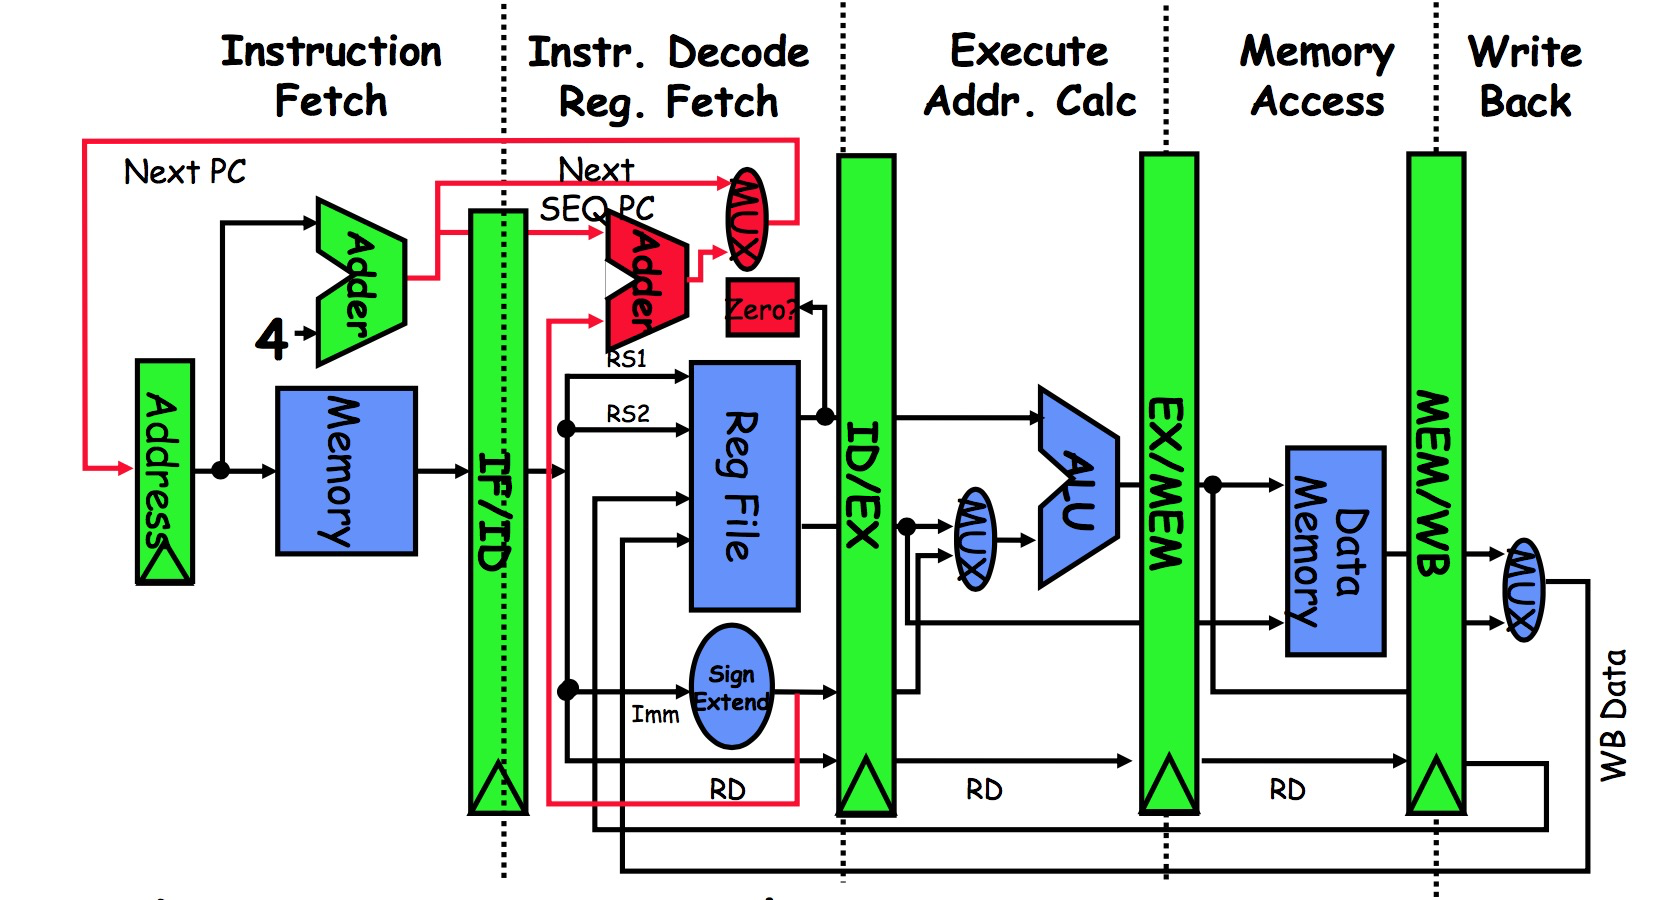
\includegraphics[width = 13 cm]{mips}
			\caption{Five-Stage MIPS Pipeline}
			\label{fig::mips}
		\end{figure}
		So my project contains five stage modules: \verb|stage_if.v|,\verb|stage_id.v|,\verb|stage_ex.v|,\verb|stage_mem.v| and \verb|stage_wb.v|
		, four transition buffers:\verb|trans_if_id.v|,\verb|trans_id_ex.v|,\verb|trans_ex_mem.v| and \verb|trans_mem_wb.v|, one regitser file: \verb|register.v|\\
		And there is a \verb|cpu.v| to build connections between thse modules.
	\subsection{Memory}
		In this project, Harvard Architecture is used. So I have \verb|rom.v| for instructions and \verb|ram.v| for other data.
	\subsection{SOPC}
		In this project, I use \verb|sopc.v| to build connections between memory and cpu(the pipeline).
\section{Hazard and Solution}
	\subsection{RAW Hazard}
	In this project, only RAW(Read After Write) is possible to happen. It means that some instruction being decoding wants to read data from a register that is  destination of an ealier instruction when the result hasn't been written into the register.
	\subsection{Solution for RAW Hazard}
		\subsubsection{Forwarding}
			If after excution stage, the result to be written into the destination register has been got, send this result to instruction decoding stage. And instruction decoding stage can estimate whether it can use this result. The major structure is shown in \ref{fig::forwarding}
			\begin{figure}[H]
				\centering
				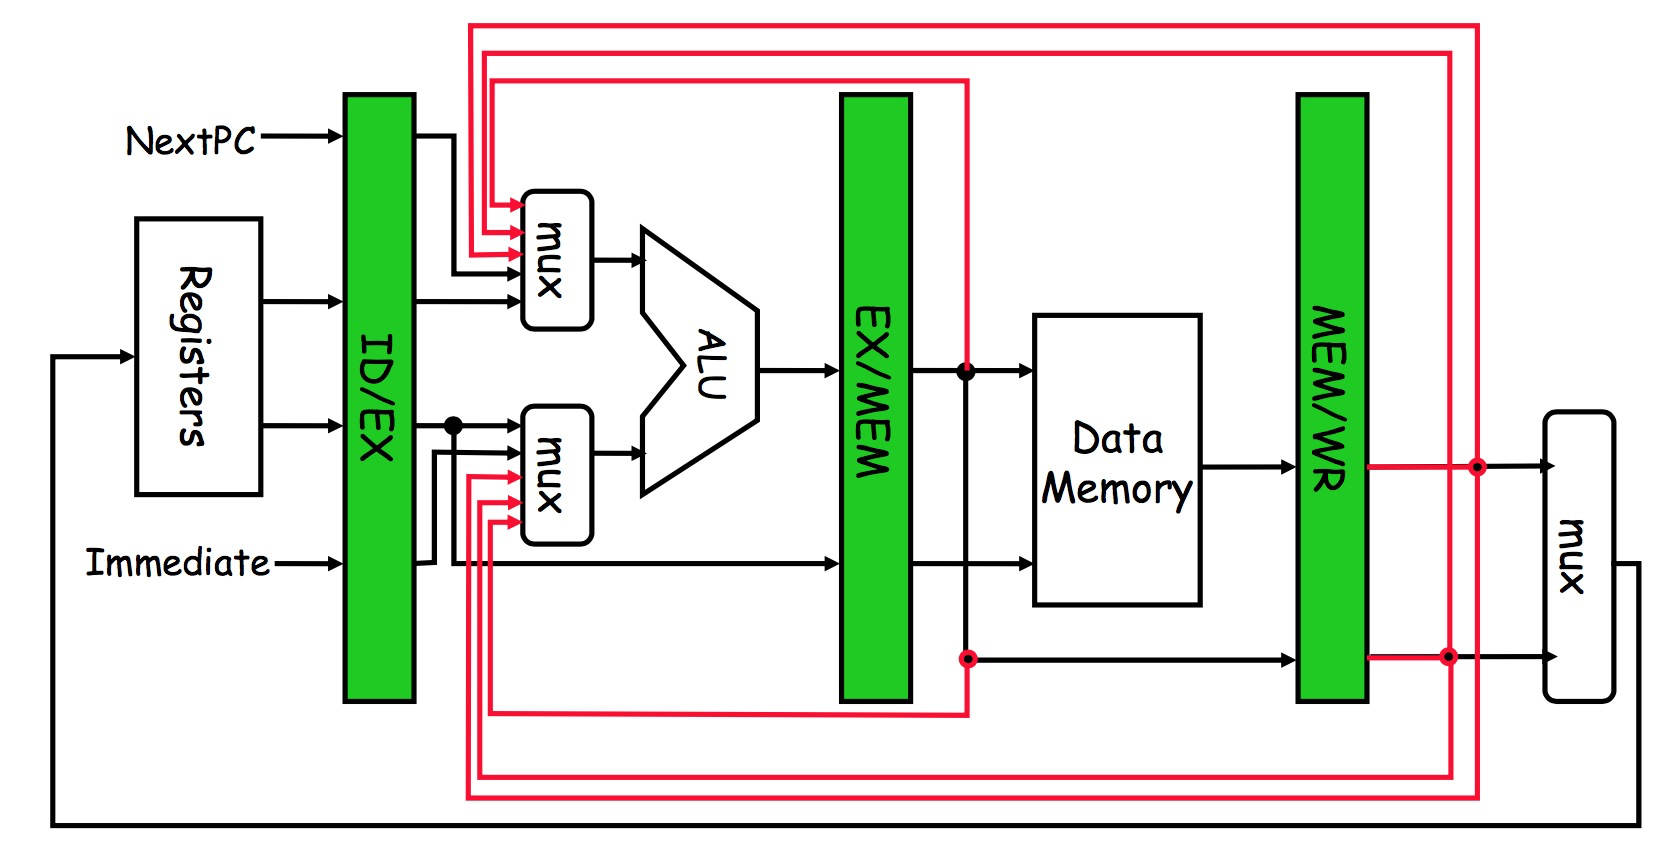
\includegraphics[width = 13 cm]{forwarding}
				\caption{Forwarding}
				\label{fig::forwarding}
			\end{figure}
			
		\subsubsection{Stall}
			There can be some situations that RAW happens even with forwardig. An example is shown in \ref{fig::stall_0}
			\begin{figure}[H]
				\centering
				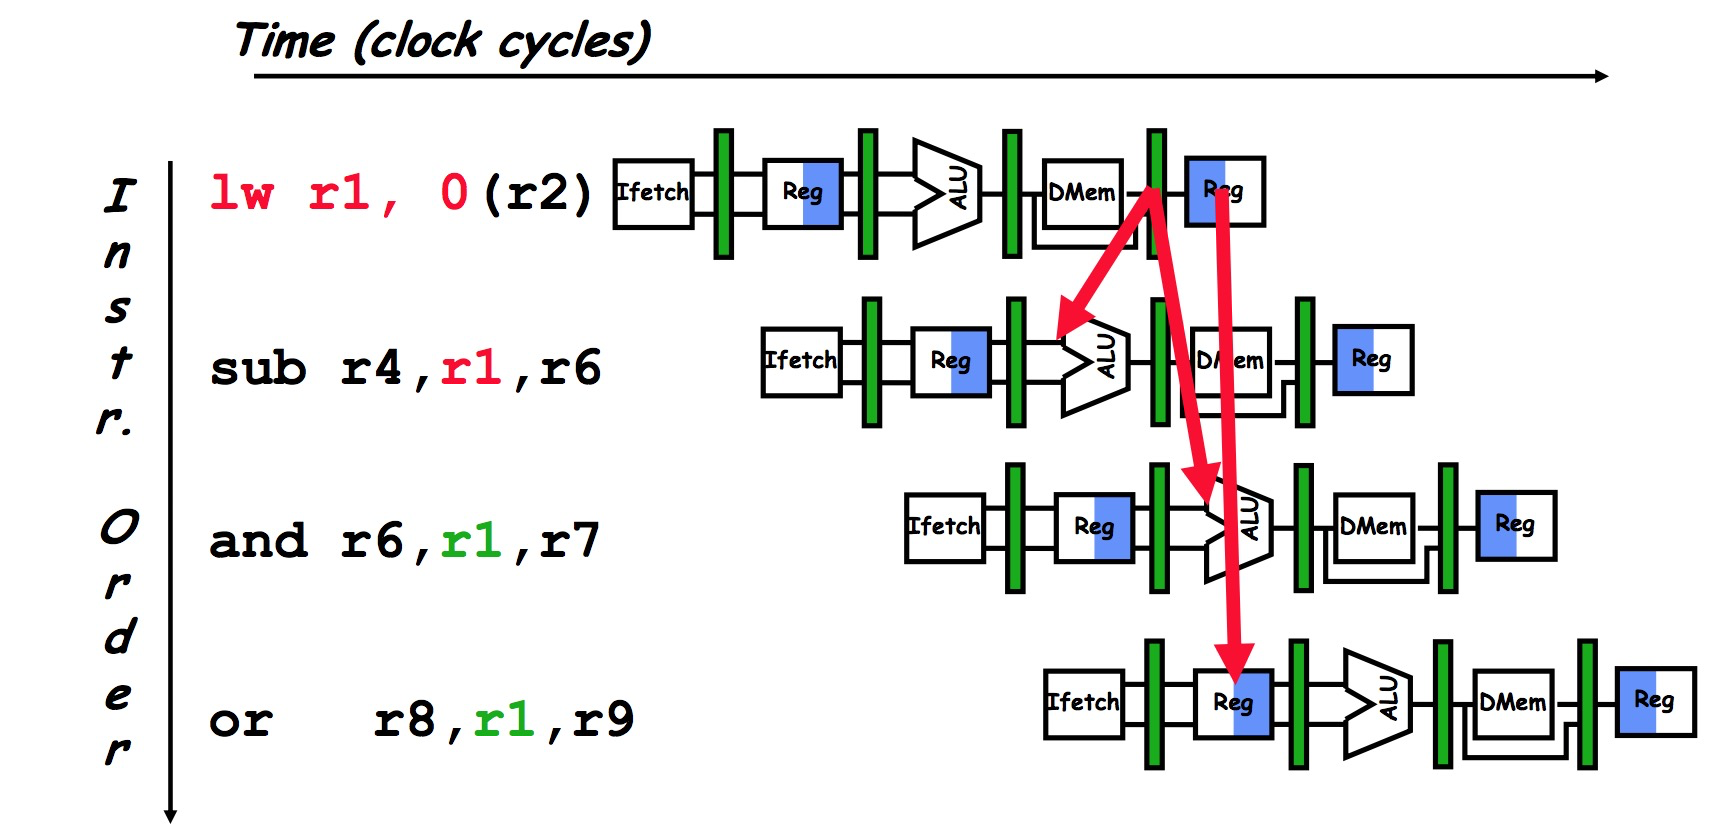
\includegraphics[width = 13 cm]{stall}
				\caption{RAW Happens Even With Forwarding}
				\label{fig::stall_0}
			\end{figure}
			To deal with such situation, we just stall all the following instructions for one cycle. 
			
\section{Main Modules Elaboration}
    \subsection{Pipeline Modules}
    	There are five stages in this five-stage MIPS pipeline.\\
    	Please refer to the code for detailed input and output of each module. I wrote some comments in the code.
    	\subsubsection{Instruction Fetch} Implemented in \verb|stage_if.v|. The main function of this module is to generate \verb|PC|, the address of current instruction, which will be sent to instruction memory (\verb|rom.v|) in \verb|sopc.v| to access instruction. And it also receive control signals to change \verb|PC|.
    	\subsubsection{IF/ID} Implemented in \verb|trans_if_id.v|. 
    	The main function of this module is to deal with stall from stage IF  and transfer data from stage IF  to stage ID. However, in this project, stall in this module will never happen.
    	
    	\subsubsection{Instruction Decode} Implemented in \verb|stage_id.v|. This module is mainly a decoder, which takes instruction from IF module as the input and outputs several control signals. Those signals are
    		\begin{table}[!htb]
				\centering
				\begin{tabular}{|l|l|}
				\hline
				\multicolumn{1}{|c|}{Signal} & \multicolumn{1}{c|}{Meaning}                                    \\ \hline
		    \verb|reg_write_enable|                  & whether or not is to write register                             \\ \hline
			\verb|reg_write_address|                       & which register is to be write                                   \\ \hline
			\verb|pc_write_enable|				&whether or not is to modify \verb|PC|								\\ \hline
			\verb|pc_write_data|				 &what to write into \verb|PC| 												\\ \hline
			\verb|mem_write_enable|                     & whether or not is to write memory                               \\ \hline
			category                      & the type of computation to perform in ALU in execution stage    \\ \hline
			operator                        & the subtype of computation to perform in ALU in execution stage \\ \hline
			\verb|operand_a|                      & the first source of ALU 				                  \\ \hline
			\verb|operand_b|                		& the second source of ALU				                  \\ \hline
			\verb|stall_request|                      & whether or not this instruction should be stalled           \\ \hline
				\end{tabular}
				\caption{A Summary on the decoder's output signals}
			\end{table}
			
			This module also output some other signals such as the original instruction and some signals to interact with register file.
		\subsubsection{ID/EX} Implemented in \verb|trans_id_ex.v|. The main function of this module is to deal with stall in stage ID, and transfer data from ID to EX.
    	\subsubsection{Execution} Implemented in \verb|stage_ex.v|. This module performs the computation except memory operation and control operation and implement forwarding.
    	\subsubsection{EX/MEM} Implemented in \verb|trans_ex_mem.v|. The main function of this module is to deal witth stall in stage EX, and transfer data from stage EX to stage MEM. However, in this project, stall in this module will never happen.
    	\subsubsection{Memory Access} Implemented in \verb|stage_mem.v|. Memory access. Receive memory instruction and output signals to interact with \verb|ram.v|. This module also implements forwarding.
    	\subsubsection{MEM/WB} Implemented in \verb|trans_mem_wb.v|. The main function of this module is to deal with stall in stage MEM, and transfer data from stage  MEM to stage WB.
    	\subsubsection{Write Back} Not implemented as a single module, since after MEM/WB, we have got all the information \verb|register.v| needs, register file can finish the write back stage.
		\subsubsection{Register File} Implemented in \verb|register.v|. The main function of this module is to simulate register storage and deal with write and read operations.
		\subsubsection{CPU} implemented in \verb|cpu.v|. This module build connections between pipeline modules above, form data path and control path.
    \subsection{Memory Modules}
    	\subsubsection{RAM}Implemented in \verb|ram.v|. This module simulates memory storage and deal with memory access.
    	\subsubsection{ROM}Implemented in \verb|rom.v|. This module simulates instruction storage and deal with instruction access.
    \subsection{SOPC Module}
    	Implemented in \verb|sopc.v|.This module build connections between Pipeline modules and Memory modules.
\section{Test Summary}
	All test code is available on \url{https://github.com/Nerer/MIPS-CPU/tree/master/test}. They are from Zhiyong Fang and Lianmin Zheng. The picture of test result is too large to display in this report. I have simulate the complex test data in presentation. So here I just show a simple example \ref{fig::sim}. We can see clearly five stages in it.
	\begin{figure}[H]
		\centering
		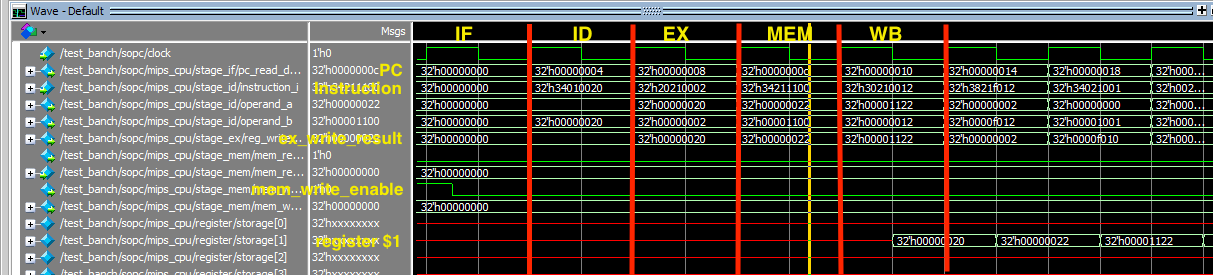
\includegraphics[width = 13 cm]{sim}
		\caption{Simulation}
		\label{fig::sim}
	\end{figure}
	
	
\section{Further Enhancement}
		Out of order execution. Traditional 5-stage MIPS pipeline is in-order execution. I think it is difficult to do improvement. Maybe we can use out of order execution such as Toma-sulo to improve the performance. But I didn't have enough time and ability to do this because I am really not familiar with Verilog.

\end{spacing}
\end{document}